\chapter{Background} \label{Ch:Background}
%=====================================================================================%
% Chapter outline:  
%    - General Introduction of the 
%       - Geology of the Delft reservoir
%           - West Netherlands Basin
%           - Reservoir stratigraphy and sedimentology
%           - Current geological conceptual model
%       - depositional environment (Delta)
%           - Delta chracteristics
%       - Current geomodelling practises
%           - Modelling approaches
%           - conditioning
%       - Machine Learning
%           - Deep learning
%           - ML in the subsurface
%       - Summary
%=====================================================================================%
% General Introduction of the Delft Reservoir amd doublet system.
The data used in this report comes from the Delft Geothermal Reservoir, located at the Delft University of Technology Campus in the Netherlands. 
As of Februari 2026 there is a doublet actively producing geothermal heat from the reservoir (\cite{beerda2026geothermie}). 
The doublet consists of a producer (\textbf{DEL-GT-01}) and injector(\textbf{DEL-GT-02-S2}), where the producer is drilled up to a TvD of $\pm$ 2337 m and the injector to a TvD of $\pm$ 2100 m (\cite{vardon2024endofwell}). 
Designed to be a research as well as a commercial project, in both wells a large number of logs and cores were collected with additional installment of monitoring instruments both in the wells as on the surface (\cite{vardon2020geothermal} and~\cite{vardon2024endofwell}). 
The targeted layer of this project is the Delft Sandstone, a member of the Lower Cretaceous Nieuwerkerk formation in the West Netherlands Basin (WNB) (\cite{donselaar2015reservoir}).
% New section
\section{Geology of the Delft Reservoir}
% Context of the West Netherlands basin
The WNB is a 60 km wide transtensional basin in the SW of the Netherlands with NW-SE trending structural highs and depressions (\cite{ziegler1990geological} as cited in~\cite{donselaar2015reservoir}). The WNB entered an active rifting stage around the Middle-Jurassic (\cite{bodenhausen1981habitat} \&~\cite{den1996fluviomarine} as cited in~\cite{willems2020geology}) leading to the formation of several half-grabens, later filled with terrestrial sediments sourced from neighboring regions (\cite{den1996fluviomarine}). the overall trend during the deposition of sediments fills in the halfgrabens led to a change in depositional environment: a transgressing shoreline moving the depositional environment from a fluvial to marine system. The Nieuwerkerk formation consists of three members: the Alblasserdam member, Delft Sandstone member (DSST) and Rodenrijs Claystone member. According to~\cite{devault2002tectonostratigraphy}, the Alblasserdam member was deposited in a fluvial environment with stacked fluvial channels and floodplain deposits. The DSST directly overlays the Alblasserdam and consists of thick stacked channel sandstone deposits with high net-to-gross values (\cite{willems2020geology};~\cite{mijnlieff2020introduction} and~\cite{bruining2023sedimentological}). The DSST is overlain by the Rodenrijs Claystone member which is rich in organics with characteristics of a lagoonal deposit (\cite{willems2020geology} \&~\cite{devault2002tectonostratigraphy} as cited in~\cite{bruining2023sedimentological}).\\
% Reservoir Stratigraphy & sedimentology
Based on recent research by~\cite{bruining2023sedimentological}, who analysed the cored section of \textbf{DEL-GT-01} and sidewall cores of \textbf{DEL-GT-02-S2}, six distinct lithofacies types could be determined. Eventually three facies associations were constructed:
\begin{itemize}
    \item \textbf{FA1:} Fluvial and distributary channel deposits.
    \item \textbf{FA2:} Crevasse spays and levee deposits.
    \item \textbf{FA3:} Overbank deposits and paleosols.
\end{itemize}
The FA1 facies is characterized by sediments that are primarily light grey fine to medium-grained sandstones that feature low-angle cross-bedding and ripple lamination with unit thicknesses ranging from 5 - 80m. FA2  is composed of well to moderately sorted, very fine to medium-grained sandstones interbedded with very dark grey siltstones and unit thicknesses ranging from 1 to 5 metres. Finally, the FA3 association consists of dark grey to very dark grey siltstone, claystone, and very fine-grained sand deposited in low-energy environments. This association  is uniquely characterised by an abundance of organic material, slickensides and millimetre-sized siderite nodules often found at the base of sequences.\\
% Current conceptual model
The depositional environment in which the DSST member was deposit has been varying in scientific literature. The DSST is attributed to both a fluvial-meandering environment (\cite{donselaar2015reservoir};~\cite{vondrak2018reservoir} \&~\cite{willems2020geology}) as well as a fluvio-deltaic system (\cite{van1993stratigraphic};~\cite{weert2024multiple} \&~\cite{bruining2023sedimentological}). With the report by~\cite{bruining2023sedimentological} having anlysed all the available cores of the \textbf{DEL-GT-01} and \textbf{DEL-GT-02-S2} boreholes leads to the most recent hypothesis that the \textit{cored section} of the DSST geothermal reservoir in Delft originates from a Deltaic environment of deposition. Only the first 80m of the DEL-GT-01 well is cored, amounting to $\pm$1/4th of the full well, with result that the rest of the section might leap into a different depositional environment.\\

\section{Depositional Environment}
% Characteristics of a deltaic depositional environment in terms of morphology and sedimentology
Deltaic environments of deposition form at the boundary of sea and land. Clastic sediments are supplied by river systems and deposited in a radial form at the shoreline. Several variations of delta's exist based on the dominant process influencing the delta shape: River dominated, Wave dominated or tide dominated delta's (\cite{kolb1966depositional}). In order to describe characteristics of the subaerial deltaic deposits, three different subdomain are categorized (e.d.~\cite{kolb1966depositional} \&~\cite{heldreich2017challenges}): Upper Delta plain, Lower Delta Plain and subaquoes Delta... 
\begin{itemize}
    \item \textbf{Upper Delta Plain:} The upper delta plain lies above the level of effective saltwater intrusion and is unaffected by marine processes. Most of the sediments comprising this part of the delta plain originate from the migratory tendency of distributary channels, overbank flooding during annual highwater periods, and periodic breaks in the river banks, in which "crevassing" into adjacent lake basins occurs. The major environments of deposition include braided channels, meandering channels (point bars and meander-belt deposits), lacustrine delta fill, backswamps, and flood plains (swamps, marshes, and freshwater lakes).
    \item \textbf{Lower Delta Plain:} The lower delta plain lies within the realm of river-marine interaction and extends landward from the shoreline to the limit of tidal influence. Most commonly in this environment, channels become more numerous and often show a bifurcating or anastomosing type of plan view pattern. Environments between distributary channels comprise the largest percentage of the lower delta plain and consist of actively migrating tidal channels, overbank splays (natural levees), interdistributary bays, bay fills (crevasse splays), marshes, and swamps. The major environmental sequences described consist of bay-fill deposits (interdistributary bay, crevasse splay-natural levee, and marsh) and abandoned distributary-fill deposits.
\end{itemize}
% Figure
\begin{figure}[!h]
    \centering
    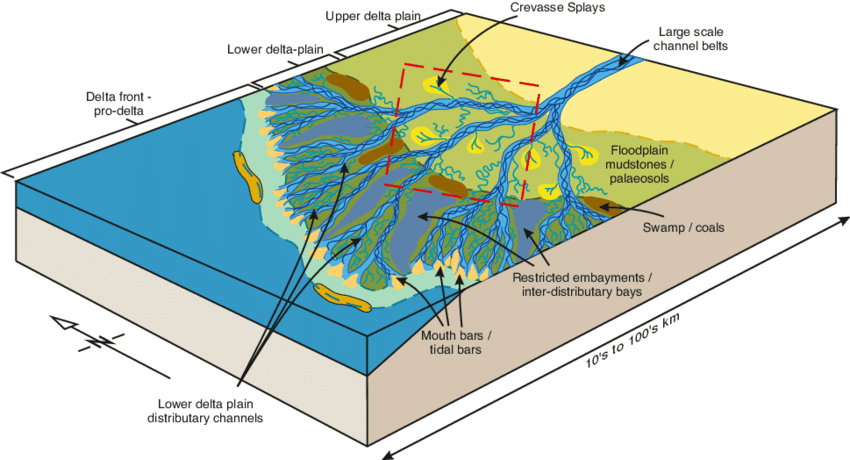
\includegraphics[width=0.85\linewidth]{figures/Upper_lower_Delta_Heldreich_2017.png}
    \caption{Example of depositional model of the Mungaroo Formation (North West Shelf, WA, Australia) highlighting the different geometries and definitions (\cite{heldreich2017challenges}).}
    \label{fig:UpperLowerDelta}
\end{figure}
% New section
\section{Geo-modelling}
The general purpose of 3D reservoir models is to provide a 3D representation of the subsurface which also allows for reservoir simulations to be performed making informed decisions possible. The model can be be updated as new information becomes available, making it essential for predicting reservoir behavior over the course of the reservoir's lifetime (\cite{emerick2025ensemble} \&~\cite{ringrose2016reservoir}). 

~\cite{koltermann1996heterogeneity} categorized existing models into three different main techniques: object-based, process-based and descriptive/geostatistical models. Where object-based models mostly ignore physics to directly place geological features, discrete models use spatial statistics for interpolation. In contrast process-based models are based on fundamental laws of conservation of mass and momentum to simulate the creation of geological features. Each model has unique advantages and disadvantages. As a result, over the past decades research has been oriented at combining different models to leverage each models advantages creating so called ~'Hybrid models' (e.g.~\cite{koltermann1996heterogeneity};~\cite{lopez2009process};~\cite{michael2010combining}). 
% New section
\section{Deep Generative modelling}
% Overview of Deep learning Practises

% 3D Geological modelling using Deep learning techniques

\section{Summary}
